\documentclass[11pt]{article}
\newcommand\tab[1][0.5cm]{\hspace*{#1}}

\usepackage{fancyhdr}
\usepackage{extramarks}
\usepackage{amsmath}
\usepackage{amsthm}
\usepackage{amsfonts}
\usepackage{tikz}
\usepackage[plain]{algorithm}
%\usepackage{algpseudocode}
\usepackage{amssymb}
\usepackage{enumitem}
\usepackage{relsize}
\usepackage{textcomp}
\usepackage{graphicx}
\usepackage{bm}
\usepackage{wasysym}
\usepackage{hyperref}
%\usepackage{textcomp}
%\usepackage{tabularx}
\usepackage{xcolor,colortbl}

\usepackage{makecell}

\definecolor{codegreen}{rgb}{0,0.6,0}
\definecolor{codegray}{rgb}{0.5,0.5,0.5}
\definecolor{codepurple}{rgb}{0.58,0,0.82}
\definecolor{backcolour}{rgb}{0.95,0.95,0.92}

\newcommand{\titledate}[2][2.5in]{%
	\noindent%
	\begin{tabular}{@{}p{#1}@{}}
		\\ \hline \\[-.75\normalbaselineskip]
		#2
	\end{tabular} \hspace{1in}
	\begin{tabular}{@{}p{#1}@{}}
		\\ \hline \\[-.75\normalbaselineskip]
		Date
	\end{tabular}
}

%\titleformat{\section}{\normalfont\Large\bfseries}{}{0pt}{}

% for forcing tables to fit
\usepackage{changepage}

\begin{document}
	

\begin{titlepage}
	
\author{Eric Pereira}
\date{December 6\textsuperscript{th}, 2019}
\title{Discrete Mathematics: Final Project}

\maketitle

\end{titlepage}

%\titlecontents{section}[0em]
{\vskip 0.5ex}%
{\scshape}% numbered sections formattin
{\itshape}% unnumbered sections formatting
{}%

\tableofcontents

\newpage \pagenumbering{arabic}

\section{Abstract}
\tab In this report I will be describing the use of Discrete Mathematics in a real life scenario, specifically focusing on the use case of Alan Turing in World War II. Alan Turing is the Mathematician, and arguably the father of computer science, and was credited for coming up with a code breaking tool to decipher the famous Enigma code used by Nazi Germany.  

\section{What is the Enigma Code?}
\tab The Enigma code was a type of cipher used to turn German documents, radio transmissions, and other forms of communication into what seemingly looks like random letter's. The way the Enigma code works is a single character value is directly connected to another letter value.

\tab The Nazi's used a machine to translate language into this code, this machine being called the Enigma Machine. The Enigma Machine would translate each letter into another letter and would encode and decode messages. It would do this through a complex series of changes and letters. Primarily, it would start by translating a letter to a corresponding paired letter via a plugboard. For example I could pair `A'-`C' so that any `A' would turn into a `C' and any `C' would turn into an `A'. There could be up to 13 pairs, but it was typically the military standard to only have 10 coupled letters. You have 26 factorial letter choices over 10 factorial letter combinations, and 6 factorial single letters. You also have to consider duplicates of the letter combinations (for exapmle `A'-`C' is the same as `C'-`A') following the ideas of inclusion and exclusion. This math would look like:
\begin{align*}
	&PlugBoard: &\dfrac{26!}{6!10!2^{10}}=\bm{150,738,274,937,250}
\end{align*}

\tab So, if I select the letter A it initially correlates to Z, B to Y, and so on for each letter. From here the code will go be translated by translating through 3 rotors, chosen of 5 rotors, with a total of 26 positions in each rotor. You can follow the product rule with the rotors in the enigma code, and you can follow a similar rule for the 26 positions on the rotor which would mean:
\begin{align*}
	&Rotor: &5*4*3=\bm{60} \\
	&Positions: &26^3=\bm{17,576}
\end{align*}

\tab Following all the math, we can completely multiply all the different parts together to see the combinations possible based on the aforementioned parts necessary to create the Enigma Machine. The mathematics behind this would look like:
\begin{align*}
	&PlugBoard*Rotor*Positions \\
	&150,738,274,937,250*60*17,576=\bm{158,962,555,217,826,360,000}
\end{align*}

\tab This is a ridiculously large number, way out of the scope of reasonably trying to brute force solve it. Now, with following the code, I could translate a message and send that message to someone. If they use the same rotor combination, letter combination, and initial rotor positions if they type in my coded message on their machine it will output the proper message, which is quite an interesting machine. A great diagram can be found at \url{ciphermachines.com}. Here is the example found:

\begin{center}
	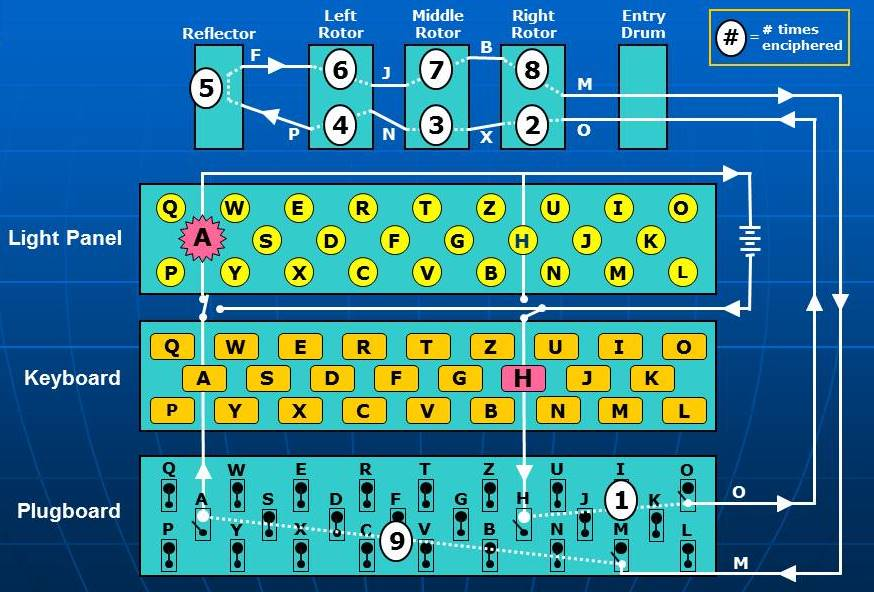
\includegraphics[scale=.5]{photos/wiring.png} \\
	\textit{Fig. 2.1}
\end{center}

\tab To add on, with the complexity of the Engima Machine as you continue to type your message the rotors will rotate, which means that the code will, essentially, change with each button press. This means that If I were to press a letter two times in a row it would actually translate to different letters each time. With this feature, the incredible difficulty of cracking it based on the specific set up of the machine, the Nazi's, and many of the Allies thought the code was impossible to crack.  

\section{How was the Enigma Code Cracked?}

\tab There was one key flaw with the Enigma system that was discovered by Alan Turing. This flaw, correlates to what was last stated about the Enigma Machine. The letter translated will be different each time you press it, except the input letter is never equal the output letter. This means that if I input the letter `E' I will never get the output letter 'E' irregardless of all my settings. 

\tab To start, you would have to make a guess of what word may be in the message. A simple and easy, tool that the Allies used is they would get a German weather report in the morning, and try to find a word that could correlate to `wetter' (`weather' in German). One way to help you deduce the position of the word is by aligning the word `wetter' with a message by checking to see if the letters are aligned or not. I.E:

\begin{center}
	\texttt{J F W I L S F T T W Q R E J \\
	            W E T T E R}
\end{center}

\tab Would not be a valid position to check because one of the T's in the encoded message lights up with `wetter', which helps us know that it is a wrong position. A position that is more possible is available if you shift left one, as so:

\begin{center}
	\texttt{J F W I L S F T T W Q R E J \\
		W E T T E R  <<<}
\end{center}

\tab From here they would have to make assumptions about the rotor configuration, plug board settings, and rotors used. So Alan Turing would come up with a plug board setting. Now, the first assumption that would be made is the plug board configuration. We can start by drawing a small diagram to describe exactly how the machine works. The machine initially takes your input, translates it through the plugboard, goes through the rotors, goes back through the plugboard and is finally output to the user. A simple chart would look like:

\begin{center}
	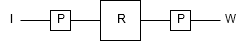
\includegraphics[scale=1]{photos/Enigma1.png}\\
	\textit{Fig. 3.1}
\end{center}

\tab This is a graph where P blocks stand for plugboards and R blocks stand for rotors. 

\tab as you can see we know what the input and output value is. From here we make an assumption about what `I' is paired to, let's start by saying `I' is paired to `A'. With our initial guessed rotor settings we have:

\begin{center}
	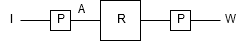
\includegraphics[scale=1]{photos/Enigma2.png}\\
	\textit{Fig. 3.2}
\end{center}

\tab From here we can keep clicking on, knowing that `I' can never output `I' we can make safe guesses of different paired letters. For example: with our initial rotor setting we may get:

\begin{center}
	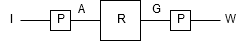
\includegraphics[scale=1]{photos/Enigma3.png}\\
	\textit{Fig. 3.3}
\end{center}

\tab As a result of this we can assume that the letter G and W are paired together. From here we can continue on and see what letters would have been paired. Let's continue on from here:

\begin{center}
	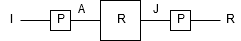
\includegraphics[scale=1]{photos/Enigma4.png} \\
	\textit{Fig. 3.4}
\end{center}
\begin{center}
	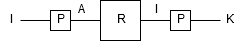
\includegraphics[scale=1]{photos/Enigma5.png} \\
	\textit{Fig. 3.5}
\end{center}

\tab the first chart pairs letter `J' and `R' but the next chart gives us a problem. The rotor output gives us `I' and with the plugboard output being `K'. This is a problem because we already coupled `I' with `A'. Because we found this flaw, we have to throw out the idea of `I' being paired with `A' and move to `I' and `B' and test that out. If we end up running out of letters we try a new rotor position, and restart with `I' and `A'. The math behind this would then, ideally, be significantly less comparisons than the expected amount. 

\tab With the guessed position you would have 60 possible rotor combinations and 17,576 rotor combinations with the guessed letter and letter position in the phrase. Following the pigenhole principle there are only 16 guesses maximum that you could make for each letter combination because we know that 10 plugs on the plugboard are plugged in and 6 are not. This means that if you have more than 10 pairs as a result of testing you know that it is wrong, and if you have 16\textsuperscript{th} that doesn't work you are also wrong. this can also occur for each instance of the 26 letters that are paired with your guessed letter. The math would work out as:
\begin{align*}
	26^4*15*17,576=\bm{128,508,962,816}
\end{align*}

\tab The number 128,508,962,816 is the maximum number of attempts possible before getting the correct guess. It is the maximum number because it is the total amount of guesses possible before a repeat guess, following the pigeonhole principle. This is significantly less guesses than the expected number mentioned in the previous section, this number of processes can be done on a modern computer processor in about 4 seconds. Of course, they did not have computers this powerful back then, so they had to create a machine, named the Bombe Machine, which would take about 20 minutes to figure out the code. It was necessary to be able to calculate this quickly as Nazi Germany would change their codes every day.

\tab There were small features added to make the code more efficient, by following the rules of inclusion and exclusion. For example, if you found out that the assumption you made is wrong you also know that all the pairs you discovered, for each rotor position, is also wrong. For each rotor this reduces the amount of guesses by at maximum. For example, in the previous example where we saw in \textit{Fig. 3.4} we see that `J' is coupled with `R'. We found that the entire system is not true for `I' and `A' for that specific rotor combination, therefore we can also confirm that it would be impossible for `J' and `R' to be coupled because that would only for an `I' and `A' combination. Due to this flaw, in any case where we encounter some `J' and `R' paired we can see that they don't work.

\tab Moreover, this is also true in the case with \textit{Fig. 3.5}. We find that `I' and `K' can also not be true, and as a result, can reduce our maximum total possible guesses in half. Making the guess total: $\dfrac{128,508,962,816}{2}=\bm{64,254,481,408}$.

\tab As a result, by finding a work around and significantly reducing the total amount of calculations to guess the code it, and allowed for the creation a machine that could crack the code.  
\end{document}
